% entsteht aus b durch t --> 1/\tau
%TODO: besserer Titel
\subsection{Beispiel ohne namen}
\begin{comment}
  Beginne mit
  \[ \tilde P=\tau\partial_\tau^2+2\partial_\tau-1 \]
  und gehe von $\tau$ über zu $t$ via $\tau\rightarrow\frac{1}{t}$:\\
  %TODO: rightarrow oder mapsto?
  \begin{itemize}
    \item was passiert mit der Ableitung $\partial_\tau$? Es gilt:
      \[
        \partial_\tau (f(\frac{1}{\tau}))=
        \partial_t(f)\cdot (-\frac{1}{\tau^2})=
        -\partial_t(f)\cdot t^2= %TODO: wegen klammerung?
        - t^2 \cdot \partial_t(f)
      \]
      also:
      \[
        \partial_\tau=-t^2\partial_t
        % stimmt das VZ?
      \]
    \item was ist $\partial_t(t^2\partial_t)$?
      \begin{align*}
        \partial_tt^2\partial_t &= (\partial_tt)t\partial_t\\
        &= (t\partial_t-1)t\partial_t\\
        &= t(\partial_tt)\partial_t-t\partial_t\\
        &= t(t\partial_t-1)\partial_t-t\partial_t\\
        &= t^2\partial_t^2-2t\partial_t\\
      \end{align*}
    \item was passiert mit $ \tilde P=\tau\partial_\tau^2+2\partial_\tau-1 $?
      \begin{align*}
        \tilde P &= \tau\partial_\tau^2+2\partial_\tau-1\\
        &\overset{\tau\rightarrow\frac{1}{t}}{\longrightarrow}
          \frac{1}{t}(-t^2\partial_t)^2+2(-t^2\partial_t)-1\\
        &= \frac{1}{t}t^2(\partial_t(t^2\partial_t))-2t^2\partial_t-1\\
        &= t(\partial_t(t^2\partial_t))-2t^2\partial_t-1\\
        &= t(t^2\partial_t^2-2t\partial_t)-2t^2\partial_t-1\\
        &= t^3\partial_t^2-4t^2\partial_t-1 =: P\\
      \end{align*}
  \end{itemize}
\end{comment}

Wir wollen nun den zum folgendem $P$ assoziierten Meromorphen Zusammenhang
betrachten:\\
\begin{minipage}[hbt]{0,39\textwidth}
  \[ P= t^3\partial_t^2-4t^2\partial_t-1 \]
\end{minipage}
\begin{minipage}[hbt]{0,59\textwidth}
  \begin{center}
    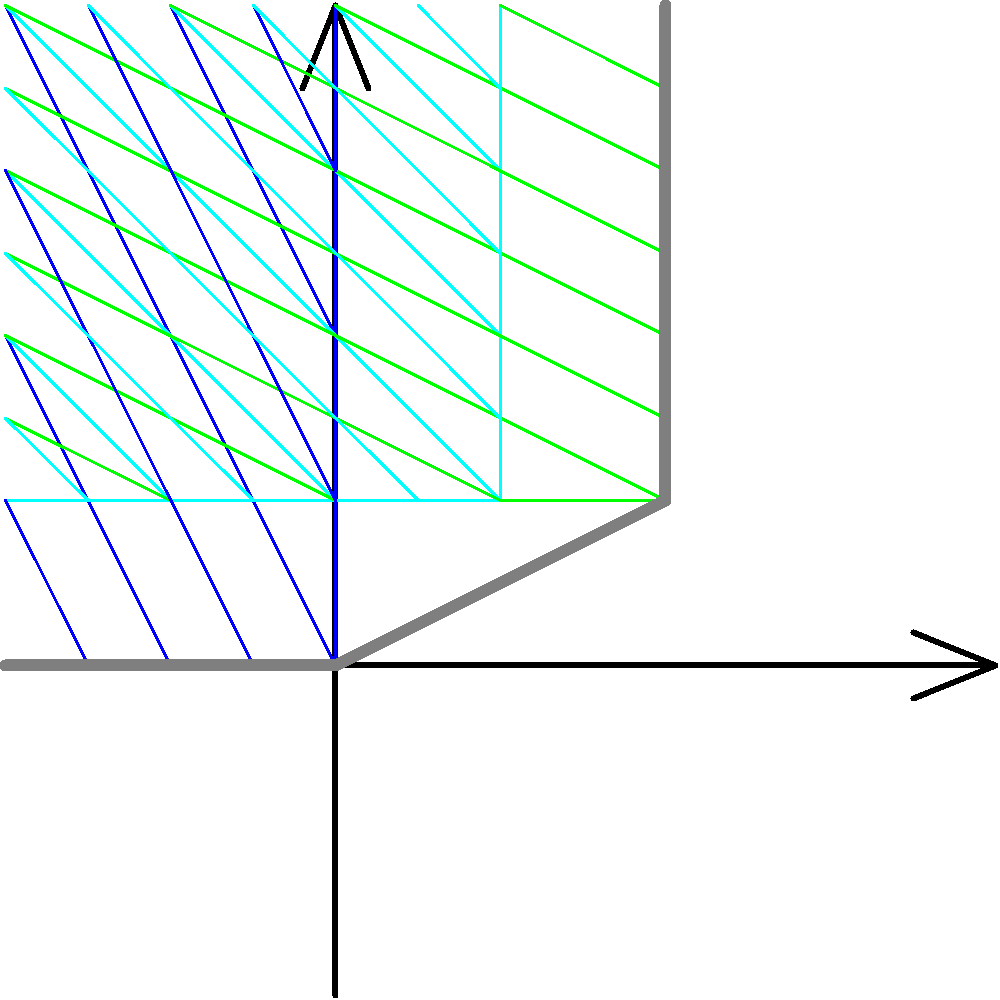
\includegraphics[width=6cm]{beispiele/img/formal_b.png}
  \end{center}
\end{minipage}
Es ist offensichtlich, dass $\slopes(P)=\{\frac{1}{2}\}$.

% vim: set ft=tex :
